\documentclass{beamer}
\mode<presentation> {
    \usetheme{Malmoe}
    \usecolortheme{whale}
    \setbeamertemplate{footline}[page number]
    \setbeamertemplate{navigation symbols}{}
}

\usepackage{graphicx} 	% Allows including images
\usepackage{booktabs} 	% Allows the use of \toprule, \midrule and \bottomrule in tables
\usepackage{tikz} 		% Pretty diagrams.
\usetikzlibrary{
    positioning				% Allows 5px above/below of x style positioning
    , arrows				% Allows <-, ->, <-> style arrows.
    , fit					% Allows fitting lines to shapes
    , decorations.pathreplacing	% Allows decoration that affect line paths.
}

%----------------------------------------------------------------------------------------
%	TITLE PAGE
%----------------------------------------------------------------------------------------

\title[Short title]{NUClear in the NUBots code}

\author{
    Trent Houliston \and Jake Woods
}

\institute[UoN]
{
    University of Newcastle \\ % Your institution for the title page
    \medskip
    \textit{Trent.Houliston@uon.edu.au, Jake.f.woods@gmail.com} % Email address
}

\date{\today}

% Start of document
\begin{document}

%----------------------------------------------------------------------------------------
% Title Slide 
%----------------------------------------------------------------------------------------
\begin{frame}
    \titlepage % Print the title page as the first slide
\end{frame}


%----------------------------------------------------------------------------------------
% Overview (Table of Contents
%----------------------------------------------------------------------------------------
\begin{frame}
    \frametitle{Overview}
    \tableofcontents
\end{frame}

%----------------------------------------------------------------------------------------
\section{Current System}
%----------------------------------------------------------------------------------------
\subsection{Existing Components}
\begin{frame}
    \frametitle{Some title}
    Some text here
\end{frame}

\begin{frame}
    \frametitle{Some title}
    Some text here
\end{frame}

\subsection{Existing Architecture}
\begin{frame}
    \frametitle{Existing Architecture}
    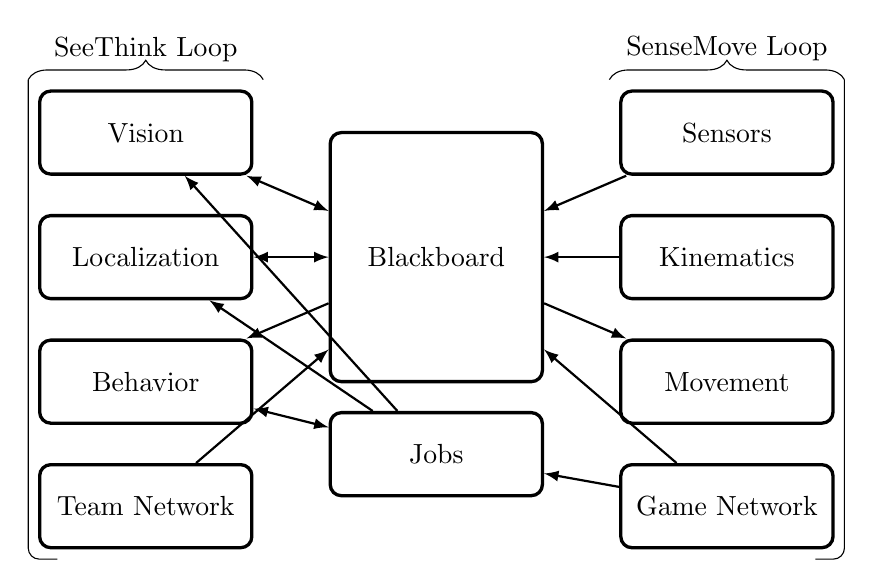
\begin{tikzpicture}[
            x=10.5em,y=4.5em,
            component/.style={
                rectangle,
                rounded corners,
                draw=black, very thick,
                text width=7em,
                minimum height=3em,
                text centered
            },
            write/.style={ ->, thick },
            read/.style={<-, thick},
            readwrite/.style={<->, thick},
            >=latex
        ]

        %\node at (0.5,2.5) {$P_{1}$};

        %%% Nodes
        %% Left hand Side
        \node at (0,3) [component] (vision) {Vision};
        \node at (0,2) [component] (localization) {Localization};
        \node at (0,1) [component] (behavior) {Behavior};
        \node at (0,0) [component] (teamnetwork) {Team Network};

        %% Center
        \node at (1, 2) [component,minimum height=9em] (blackboard) {Blackboard};
        \node [below=1em of blackboard,component] (jobs) {Jobs};

        %% Right hand side
        \node at(2,3) [component] (sensors) {Sensors};
        \node at(2,2) [component] (kinematics) {Kinematics};
        \node at(2,1) [component] (movement) {Movement};
        \node at(2,0) [component] (gamenetwork) {Game Network};

        %%% Connections
        %% Left hand blackboard connections
        \path [readwrite] (vision) edge (blackboard);
        \path [readwrite] (localization) edge (blackboard);
        \path [read] (behavior) edge (blackboard);
        \path [write] (teamnetwork) edge (blackboard);

        %% Left hand jobs connections
        \path [read] (vision) edge (jobs);
        \path [read] (localization) edge (jobs);
        \path [readwrite] (behavior) edge (jobs);

        %% Right hand blackboard connections
        \path [write] (sensors) edge (blackboard);
        \path [write] (kinematics) edge (blackboard);
        \path [read] (movement) edge (blackboard);
        \path [write] (gamenetwork) edge (blackboard);

        %% Right hand jobs connections
        \path [write] (gamenetwork) edge (jobs);

        %%% Decorations
        %% SeeThink header
        \node[fit=(vision)(localization)(behavior)(teamnetwork)](leftgroup){};
        \draw[rounded corners] 
        (leftgroup.north west)--(leftgroup.south west) -- ++(0.10,0);            
        \draw[decorate,decoration={amplitude=7pt,brace}] % Header line
        (leftgroup.north west) -- (leftgroup.north east);

        \node[above=1.1em of leftgroup,anchor=center]{SeeThink Loop};

        %% SenseMove header
        \node[fit=(sensors)(kinematics)(movement)(gamenetwork)](rightgroup){};
        \draw[rounded corners] 
        (rightgroup.north east) -- (rightgroup.south east) -- ++(-0.10,0);
        \draw[decorate,decoration={amplitude=7pt,brace}]
        (rightgroup.north west) -- (rightgroup.north east);
        \node[above=1.1em of rightgroup,anchor=center]{SenseMove Loop};
    \end{tikzpicture}

\end{frame}

\begin{frame}
    \frametitle{Some title}
    Crap
\end{frame}

%----------------------------------------------------------------------------------------
\section{NUClear Architecture}
%----------------------------------------------------------------------------------------
\subsection{Architectural Overview}
\begin{frame}
    \frametitle{Some title}
    Some text here
\end{frame}

\begin{frame}
    \frametitle{Some title}
    Some text here
\end{frame}

\subsection{Key Functions}
\begin{frame}
    \frametitle{Some title}
    Some text here
\end{frame}

\begin{frame}
    \frametitle{Some title}
    Some text here
\end{frame}

%----------------------------------------------------------------------------------------
\section{NUClear in NUBots}
%----------------------------------------------------------------------------------------
\subsection{Module Examples}
\begin{frame}
    \frametitle{Some title}
    Some text here
\end{frame}

\begin{frame}
    \frametitle{Some title}
    Some text here
\end{frame}

\subsection{Key Functions}
\begin{frame}
    \frametitle{Some title}
    Some text here
\end{frame}

\begin{frame}
    \frametitle{Some title}
    Some text here
\end{frame}

\subsection{Current Porting Status}
\begin{frame}
    \frametitle{Some title}
    Some text here
\end{frame}

\begin{frame}
    \frametitle{Some title}
    Some text here
\end{frame}

\end{document} 
